\documentclass[12pt]{article}
\usepackage[margin=1in]{geometry}
\usepackage{graphicx}
\usepackage{booktabs}
\usepackage{hyperref}
\usepackage{setspace}
\usepackage{parskip}

\onehalfspacing

\title{\textbf{Problem Set 6: Data Cleaning and Visualization} \\
       \large Econ 5253 -- Data Science for Economists, Spring 2026}
\author{Sumedha Ray}
\date{\today}

\begin{document}
\maketitle

% -------------------------------------------------------
\section{Data Description}
% -------------------------------------------------------

The data used in this problem set come from \textit{ProQuest Dissertations \& Theses Global}, a comprehensive database of doctoral dissertations. I exported a pilot sample of 100 economics dissertations completed in 2015 in RIS format. This dataset is part of a larger ongoing project examining whether PhD economists who study sensitive research topics face different career trajectories than those who do not.

Each RIS record contains bibliographic information including the dissertation title, author name, advisor name(s), year of completion, degree-granting institution, geographic location, page count, and a set of keyword tags that include both free-text descriptors and structured subject codes (e.g., \texttt{0501:Economics}, \texttt{0510:Labor economics}).

% -------------------------------------------------------
\section{Data Cleaning Steps}
% -------------------------------------------------------

The raw RIS file is a plain-text format where each field is identified by a two-letter tag (e.g., \texttt{T1} for title, \texttt{AU} for author, \texttt{PB} for publisher/university). I wrote a custom parser in R that reads the file line by line and splits it into individual records using the end-of-record marker \texttt{ER  -}. The following cleaning steps were applied.

\textbf{Field extraction.} For most fields (title, author, year, university, state, page count), only one value per record is expected. For advisor (\texttt{A3}) and keywords (\texttt{KW}), multiple lines are possible and were collected into a single string separated by semicolons.

\textbf{Subfield classification.} ProQuest encodes primary subject classifications as keyword entries of the form \texttt{NNNN:SubfieldName} (e.g., \texttt{0501:Economics}). I identified these coded entries using a regular expression and extracted the subfield label from the first match in each record. I also standardized a handful of near-duplicate labels with inconsistent capitalization (e.g., ``Agricultural economics'' and ``Agricultural Economics'').

\textbf{Sensitive topic flag.} For each record, I constructed a binary indicator equal to 1 if any keyword in that record matched a predefined list of sensitive topic terms, including race, gender, religion, discrimination, poverty, drug use, crime, and related concepts. This variable is relevant to the broader research project motivating this dataset.

\textbf{Page count cleaning.} Page counts below 10 or above 600 were coded as missing, as these likely reflect data entry errors or non-standard records (e.g., multivolume works with only one volume listed).

\textbf{Record filtering.} Two records with missing titles or missing university names were dropped, leaving a final analytic sample of 100 dissertations.

The cleaned dataset was saved as \texttt{dissertations\_clean.csv} for reproducibility.

% -------------------------------------------------------
\section{Visualizations}
% -------------------------------------------------------

\subsection{Figure 1: Top 15 Universities by Dissertation Count}

\begin{figure}[h!]
    \centering
    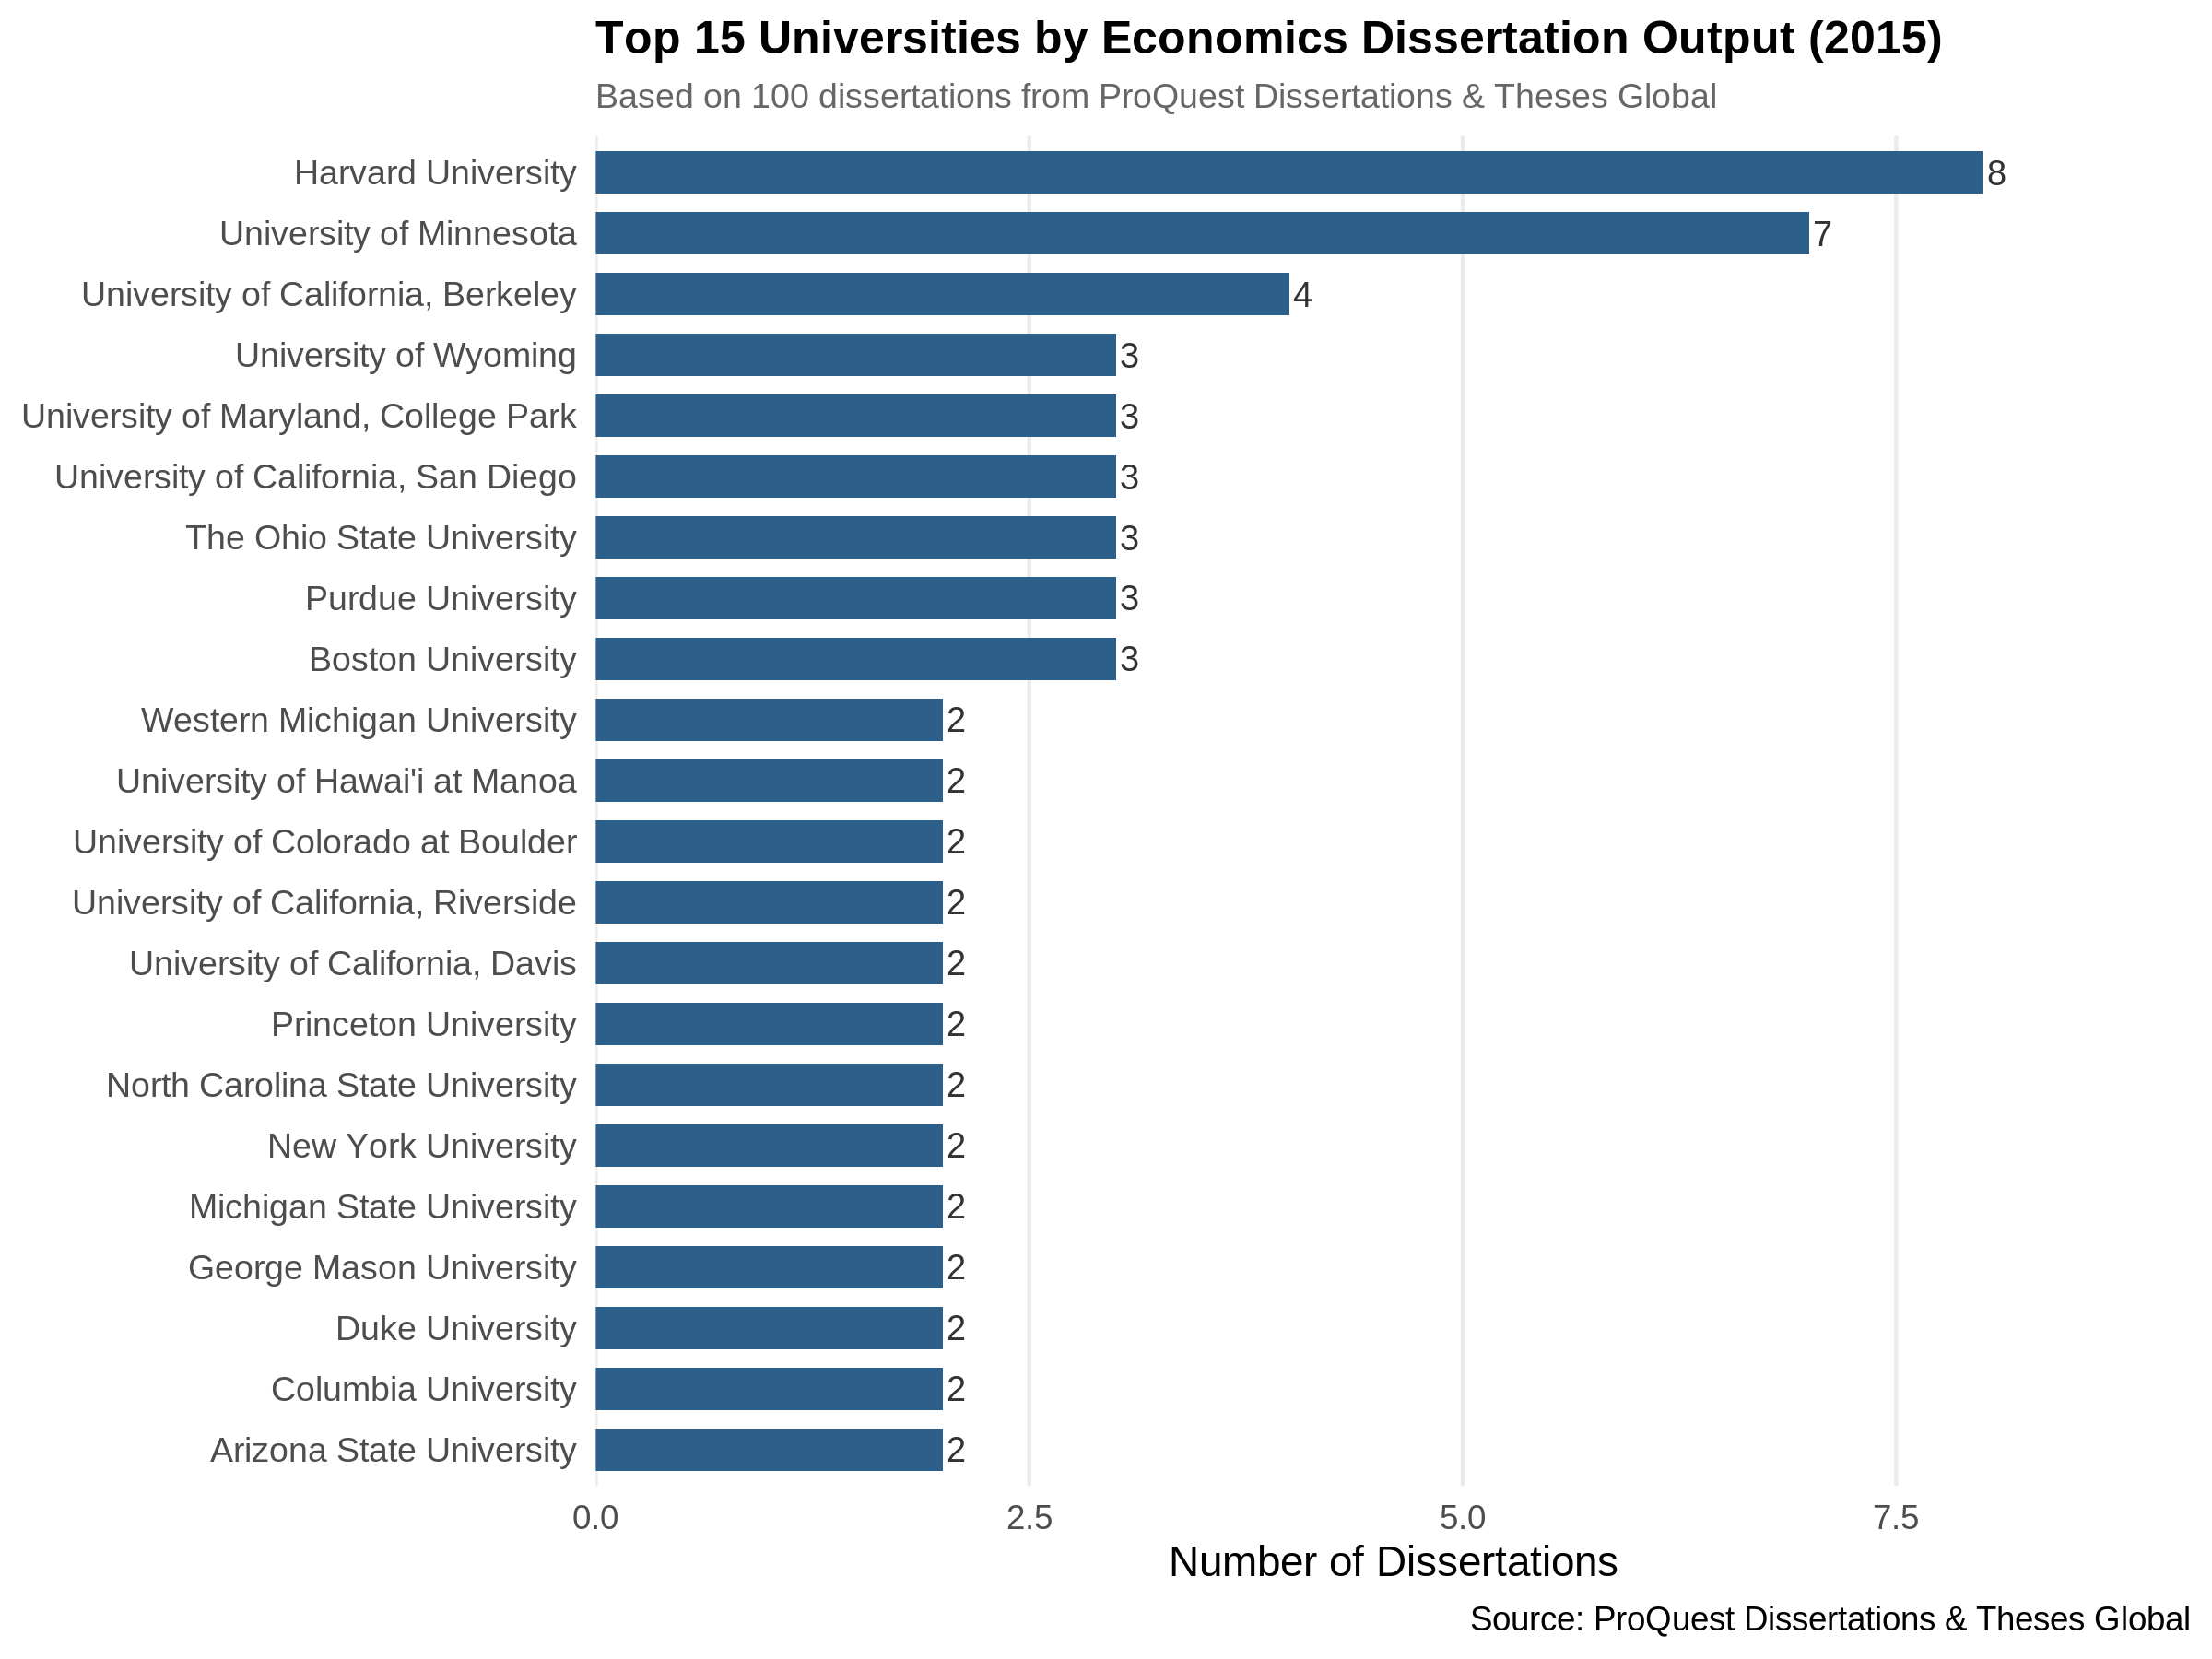
\includegraphics[width=0.92\textwidth]{PS6a_Ray.png}
    \caption{Top 15 universities by number of economics dissertations in the 2015 sample.}
    \label{fig:universities}
\end{figure}

Figure~\ref{fig:universities} shows the 15 degree-granting institutions with the highest dissertation counts in the sample. Harvard University leads with 8 dissertations, followed by the University of Minnesota with 7. The distribution is right-skewed: a small number of research-intensive universities account for a disproportionate share of PhD production. This pattern is consistent with the broader literature on the concentration of PhD training in economics, and is relevant for the job market paper project since advisor networks and institutional prestige are key covariates of interest.

\subsection{Figure 2: Dissertation Count by Subfield}

\begin{figure}[h!]
    \centering
    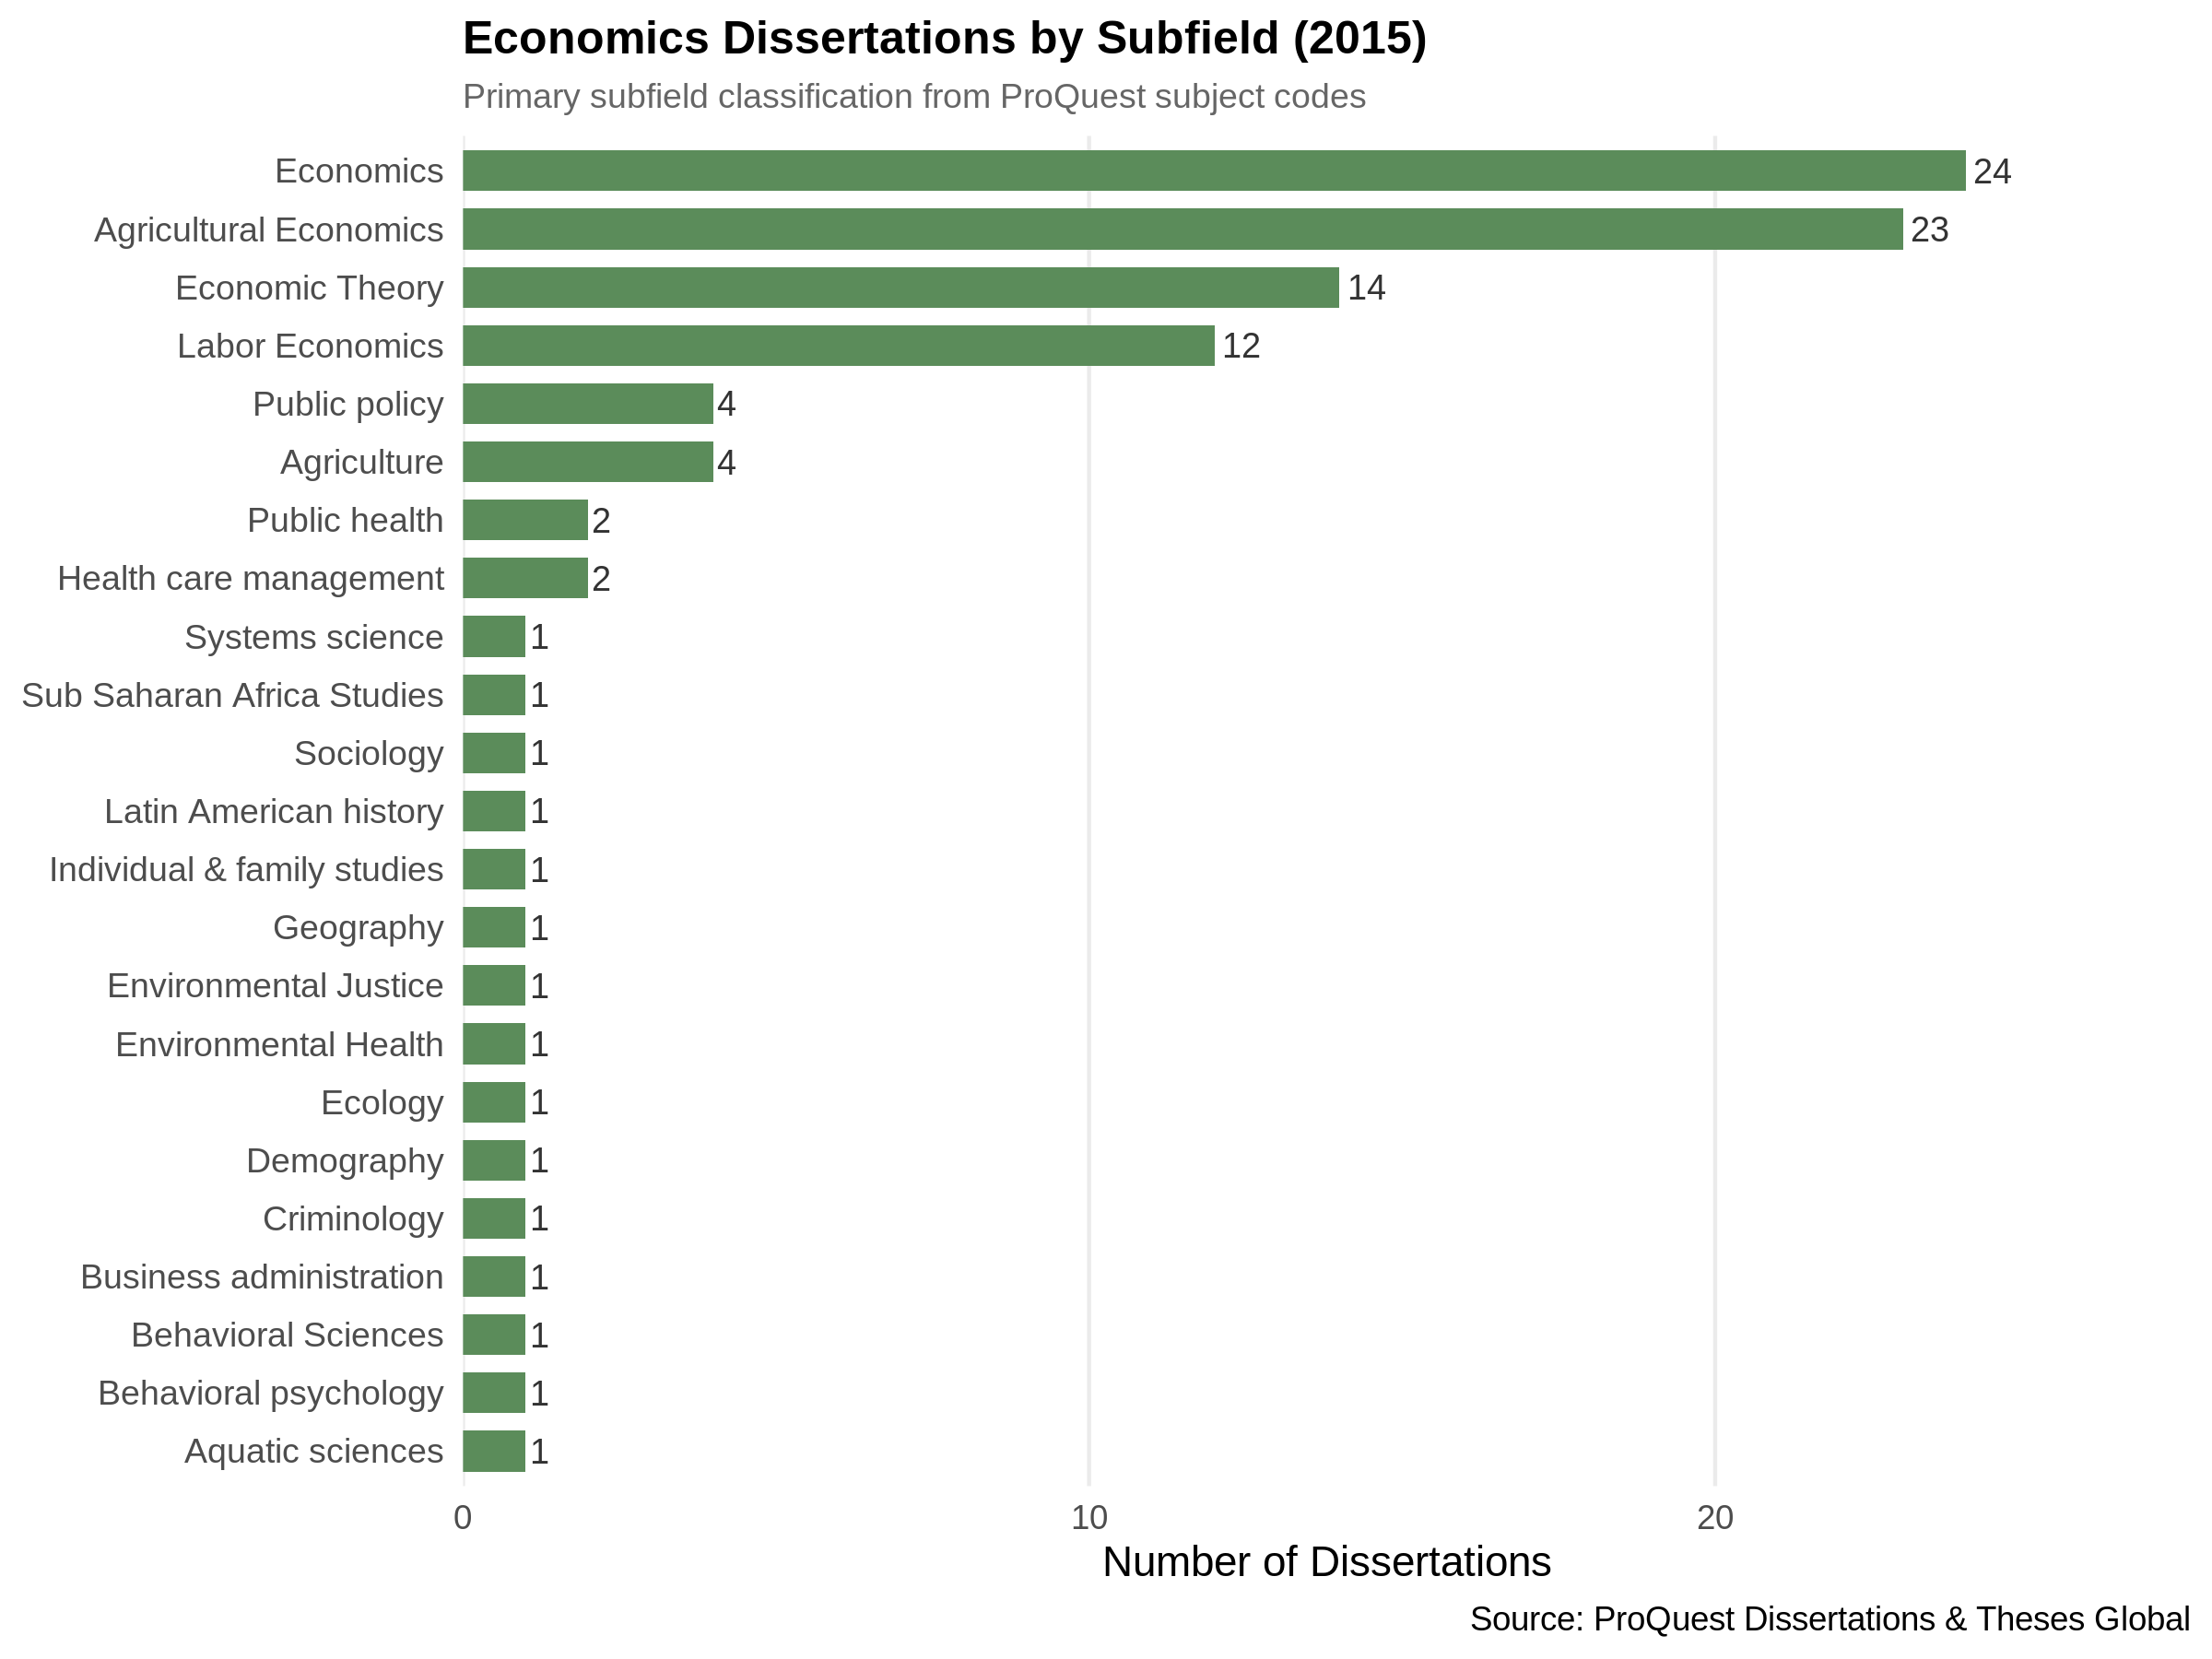
\includegraphics[width=0.92\textwidth]{PS6b_Ray.png}
    \caption{Number of dissertations by primary subfield classification (top 12 subfields shown).}
    \label{fig:subfields}
\end{figure}

Figure~\ref{fig:subfields} displays the distribution of dissertations across economics subfields as coded by ProQuest's structured subject classification system. ``Economics'' as a general category is the most common primary classification, followed by environmental economics, agricultural economics, and labor economics. The prominence of environmental and agricultural economics likely reflects the search query used to generate the pilot sample. This visualization helps characterize the topical composition of the dataset and will inform how the full-scale project stratifies dissertations by field.

\subsection{Figure 3: Dissertation Length by Subfield}

\begin{figure}[h!]
    \centering
    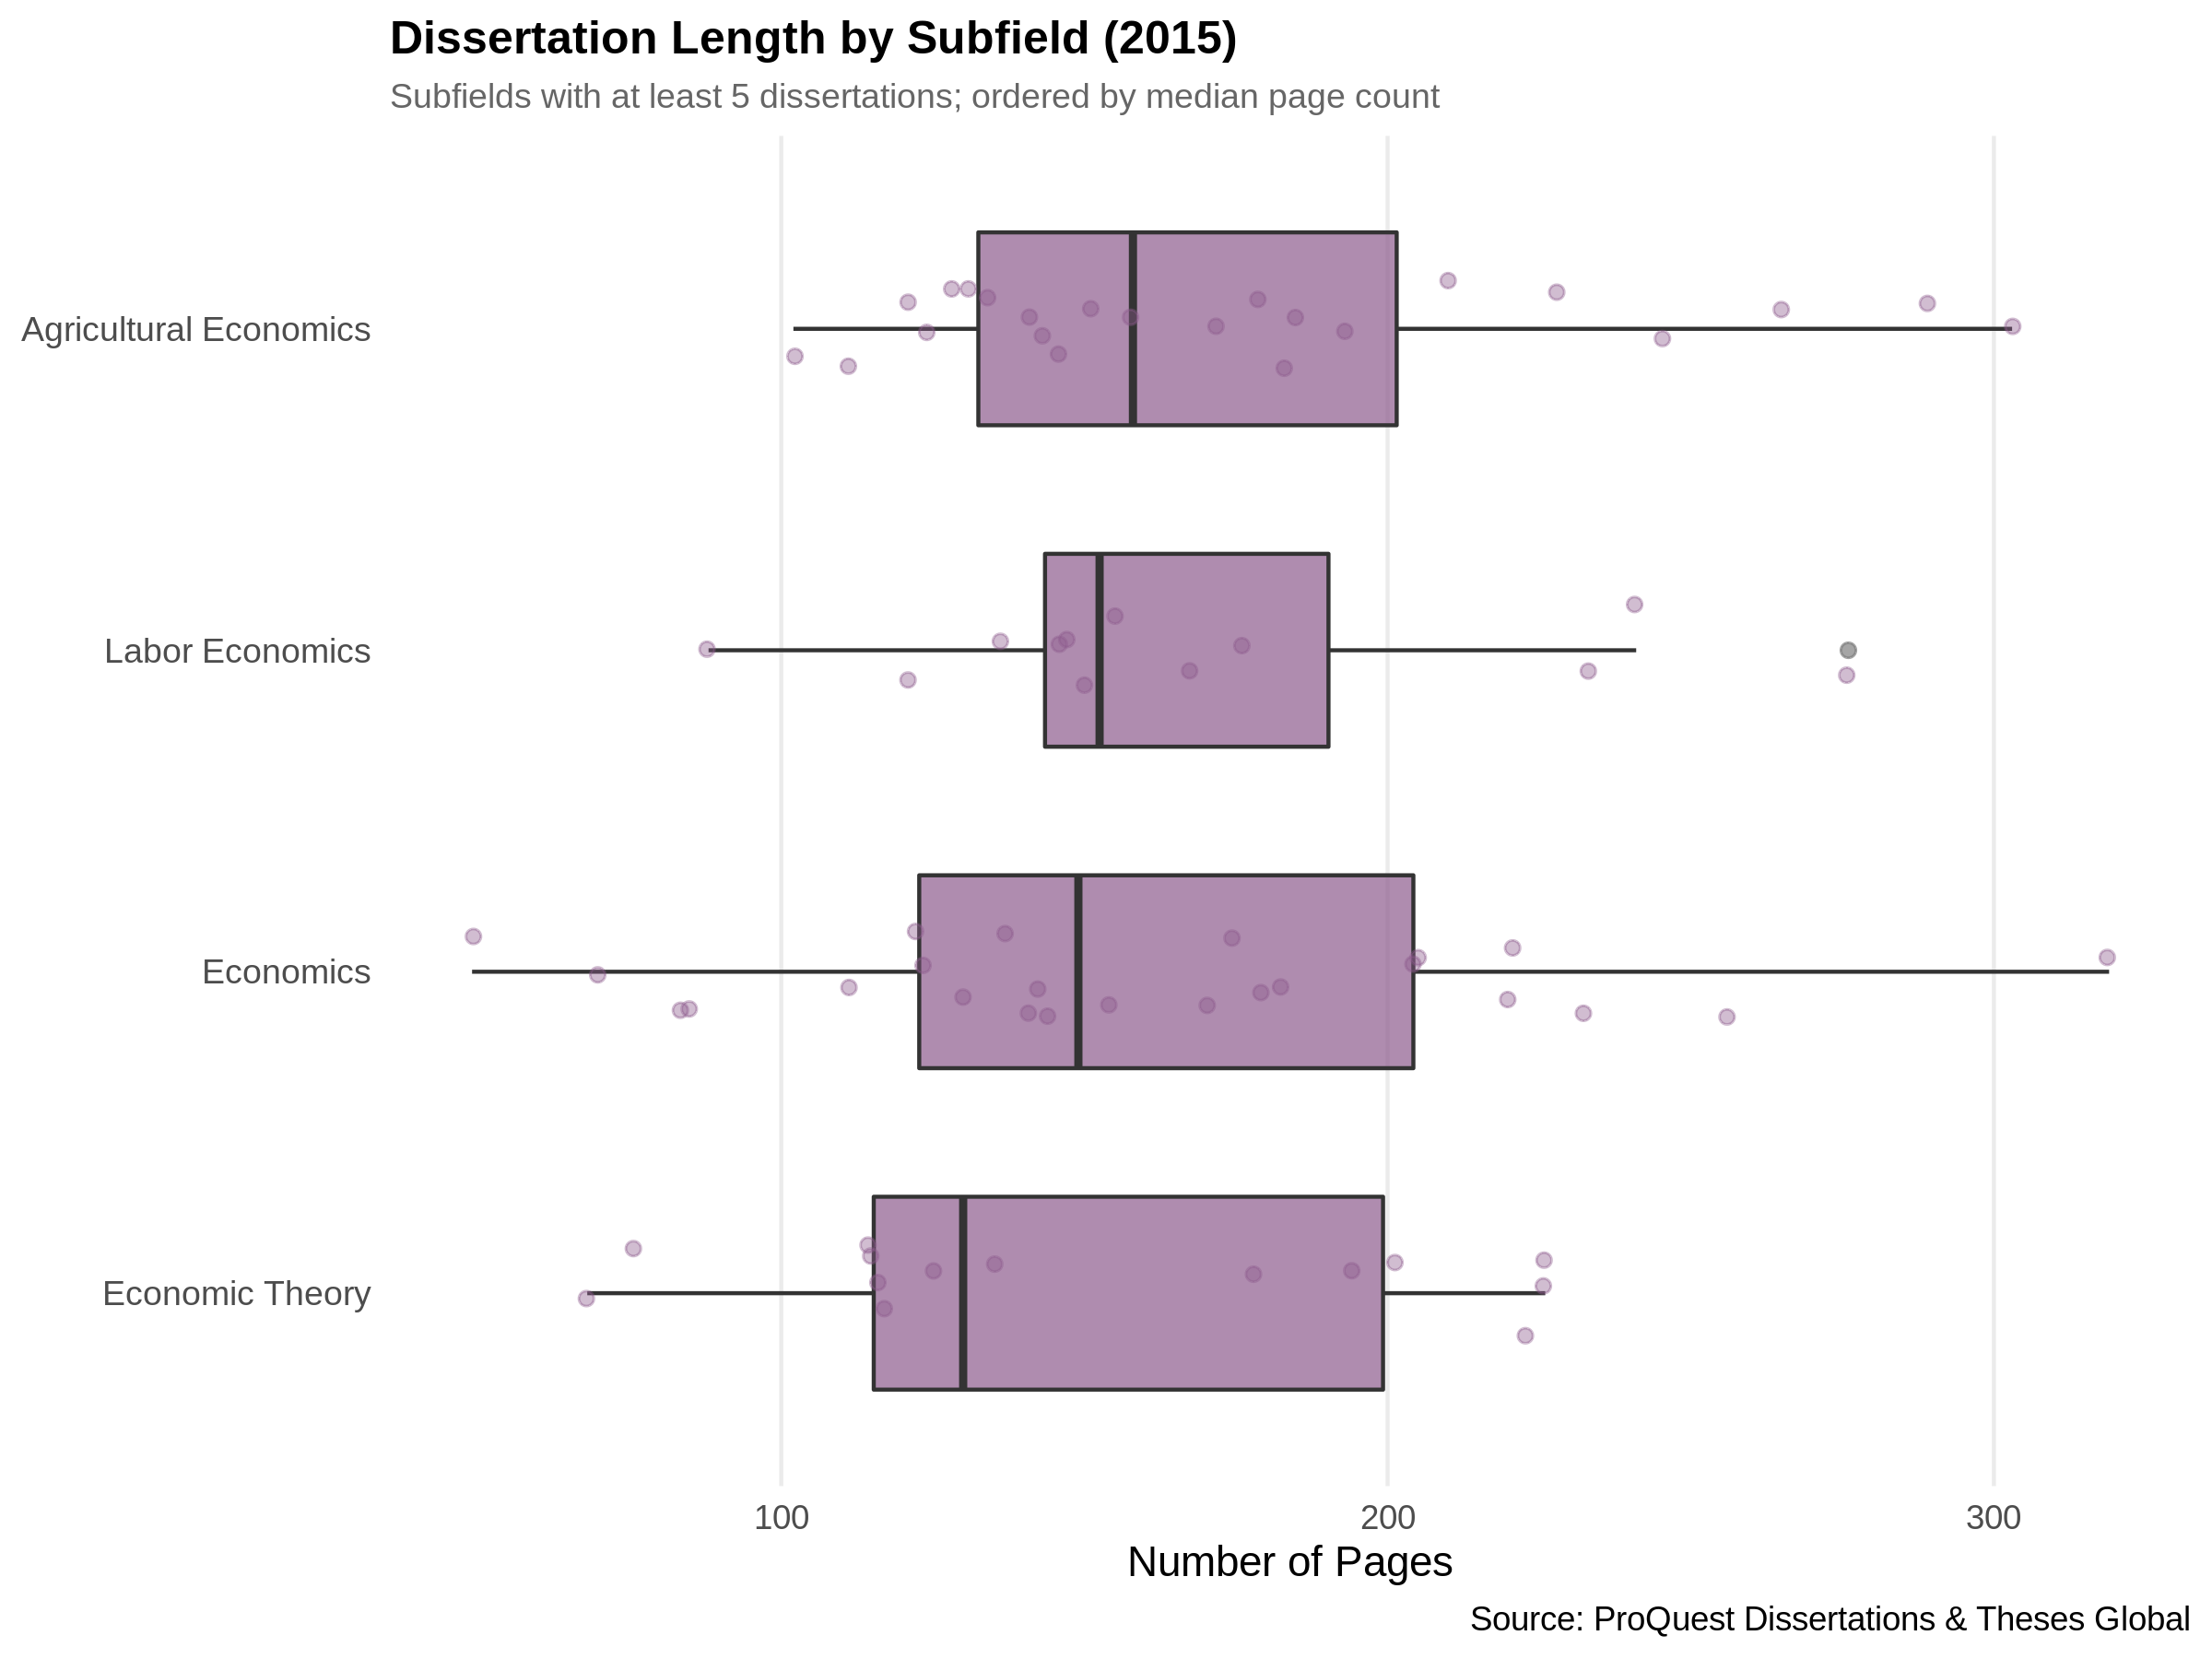
\includegraphics[width=0.92\textwidth]{PS6c_Ray.png}
    \caption{Distribution of dissertation page counts by subfield (subfields with at least 5 dissertations). Points are individual dissertations; boxes show the interquartile range and median.}
    \label{fig:pages}
\end{figure}

Figure~\ref{fig:pages} presents box plots of dissertation page counts for each subfield with at least five observations, ordered by median length. There is meaningful variation across subfields: dissertations in agricultural economics tend to be longer than those in labor economics or economic theory, potentially reflecting differences in empirical scope, data collection requirements, or disciplinary norms. The spread within subfields is also substantial, suggesting that page count is a noisy signal of dissertation scope. This variable may serve as a control in the job market paper's regression framework.

% -------------------------------------------------------
\section{Conclusion}
% -------------------------------------------------------

Together, the three visualizations reveal the institutional concentration of PhD production, the subfield composition of 2015 economics dissertations, and variation in dissertation length across subfields. These patterns provide useful descriptive context for the larger project examining career outcomes of PhD economists who study sensitive research topics.

\end{document}
